\documentclass[conference]{IEEEtran}
\IEEEoverridecommandlockouts

\usepackage{cite}
\usepackage{amsmath,amssymb,amsfonts}
\usepackage{graphicx}
\usepackage{textcomp}
\usepackage{xcolor}
\usepackage{booktabs}
\usepackage{multirow}
\usepackage{tikz}
\usetikzlibrary{arrows.meta, positioning}
\usepackage{hyperref}

\newcommand{\opt}[1]{\texttt{-O#1}}
\newcommand{\pass}[1]{\texttt{#1}}
\graphicspath{{../}{../checkpoints/}}

\begin{document}

\title{Learning LLVM Pass Sequences via Reinforcement Learning\\
with Autoregressive Policies}

\author{
  \IEEEauthorblockN{Evan Black}
  \IEEEauthorblockA{
    \textit{Department of Modeling \& Simulation}\\
    \textit{Old Dominion University}\\
    eblac013@odu.edu
  }
}

\maketitle

\begin{abstract}
Selecting and ordering LLVM optimization passes is a combinatorial problem
that conventional fixed pipelines solve only approximately.
We collected 950{,}000 random sequences across 38 benchmarks, storing
(sequence, runtime, IR features) tuples in an on-disk bench-cache that
serves both as an offline exploration corpus and a training-time lookup
cache.
Six benchmarks were selected for RL training based on sensitivity to pass
ordering and expressiveness of the pass menu.
We train two autoregressive policy architectures---a GRU and a causal
transformer (Auto-TFX)---with proximal policy optimisation (PPO) and a
learned value baseline.
Policies observe a 48-dimensional IR state encoding positional chunk-to-chunk
deltas in normalised opcode-category frequencies and metadata-reference rates.
We evaluate two return formulations: a sparse episode return that assigns
terminal speedup uniformly across all steps, and an instruction-weighted
return that distributes credit proportionally to per-step instruction
reduction.
Greedy decoding of Auto-TFX trained with episode return achieves
2--27\% speedup over \opt{3} on five of six training benchmarks
(mean 10.4\% across all six); stochastic sampling extends this to all six.
The instruction-weighted return trains with higher value-head explained
variance but produces lower mean speedup for both architectures, because
per-step IR-reduction credit is a poor proxy for runtime improvement---a
finding corroborated by a direct IR-reduction/speedup correlation analysis.
\end{abstract}

\begin{IEEEkeywords}
reinforcement learning, compiler optimization, LLVM, pass ordering,
proximal policy optimization, transformer
\end{IEEEkeywords}

% ─────────────────────────────────────────────────────────────────────────────
\section{Introduction}

\subsection{Background and Motivation}
Modern optimizing compilers such as LLVM expose hundreds of individual
transformation passes---inlining, loop unrolling, scalar replacement of
aggregates, vectorization, dead-code elimination, and many others.
A \emph{pass pipeline} is an ordered sequence of these transformations
applied to a program's intermediate representation (IR).
Order matters: inlining before constant propagation exposes more constants
to fold; loop rotation must precede loop-invariant code motion (LICM) to
fire on the canonical loop form.

LLVM's \opt{3} flag encodes a fixed pipeline tuned by compiler engineers
for average-case performance across a broad program distribution.
While effective in aggregate, this one-size-fits-all schedule is suboptimal
for individual programs: the same benchmark compiled with a different pass
ordering of equal length can run substantially faster or slower.
Finding the best pipeline for a specific program is NP-hard in
general~\cite{almagor2004finding} and has been studied as the
\emph{phase-ordering problem}.

Machine learning offers a principled alternative: learn a policy that maps
program features to pass choices, trained on real execution-time feedback.
If the policy captures which program characteristics predict the benefit of
each pass, it can generalise to unseen programs and outperform hand-crafted
schedules.

\subsection{Problem Statement}
We model pass sequencing as a finite-horizon MDP.
At step $t$ the state is a feature vector $\mathbf{f}_t \in \mathbb{R}^{48}$
derived from the LLVM IR after $t$ transformations (Section~\ref{sec:irfeatures}).
The action space contains 28 optimisation passes plus a \pass{Stop} action
(\texttt{src/llvm/pass.rs}); choosing \pass{Stop} or reaching the horizon
$K = 20$ terminates the episode.
The terminal reward is the speedup of the resulting binary relative to \opt{3}:
%
\begin{equation}
r = \frac{t_{\text{O3}} - t_{\text{policy}}}{t_{\text{O3}}}
\label{eq:speedup}
\end{equation}
%
measured as the trimmed mean of repeated \texttt{CLOCK\_MONOTONIC} executions.
A positive reward means the policy's sequence produces faster code than \opt{3}.

\subsection{Related Work}
\textbf{CompilerGym}~\cite{compilergym} provides a standardised
OpenAI Gym interface to LLVM optimisation environments, enabling reproducible
RL research; prior work in that setting targets IR-size reduction rather than
runtime speedup.
\textbf{AutoPhase}~\cite{autophase} formulates phase ordering as an MDP and
trains an LSTM policy with PPO on LLVM IR features, demonstrating speedups
over \opt{3} on the LLVM test suite.
\textbf{MLGO}~\cite{mlgo} demonstrates that a learned inlining policy deployed
inside production LLVM matches or exceeds the hand-tuned heuristic at Google
scale.
\textbf{MILEPOST}~\cite{milepost} learns a nearest-neighbour predictor from
static program features to select GCC optimisation flags, achieving consistent
speedups over \opt{3} on MiBench.

Our work differs from AutoPhase in targeting wall-clock execution time
measured with hardware timing (\texttt{CLOCK\_MONOTONIC}) rather than proxy
IR metrics, and in collecting a large offline corpus of random sequences
prior to training to characterise the reward landscape and inform feature
and architecture design.

\subsection{Dataset Description}
\label{sec:dataset}
We assembled a pool of 38 self-contained C benchmark programs spanning
diverse computational patterns: sorting and searching, numerical computation,
data-structure operations, string and compression codecs, and interpreted or
recursive workloads (\texttt{pool/}).
For each benchmark, 25{,}000 random pass sequences of length 1--20 were
sampled from the 28-pass primary menu and executed, yielding approximately
950{,}000 benchmarked (sequence, runtime, IR features) tuples stored in an
on-disk key-value store we call the \emph{bench-cache}.
Three baseline compilations (\opt{0}, \opt{2}, \opt{3}) were also recorded
per benchmark.
The benchmarking harness (\texttt{benchmarks/bench\_timing.h}) reports a
10\%-trimmed mean of 201 timed iterations preceded by 5 warm-up executions,
using \texttt{CLOCK\_MONOTONIC}.

The bench-cache serves two roles.
First, it is the offline corpus for exploratory data analysis: per-pass
impact, benchmark sensitivity, and coefficient-of-variation (CV) statistics
are computed directly from the stored tuples without re-running any binaries.
Second, during RL training it acts as a lookup cache: when an episode
generates a (function, sequence) pair already in the cache, the stored
runtime is returned immediately, avoiding redundant benchmark execution.
Six benchmarks were selected from the pool for the RL training phase
(Section~\ref{sec:baseline}).

\subsection{Overview of This Work}
We evaluate two autoregressive policy architectures (GRU and transformer)
with two return formulations (episode and instruction-weighted), trained
with PPO using a learned value baseline.
The episode return represents the natural, unbiased starting point: the only
ground-truth signal available is a real benchmark measurement, and assigning
it uniformly to all steps is the honest maximum-likelihood choice.
The instruction-weighted return is a principled credit-assignment refinement
that redistributes the terminal reward using per-step information already
available in the IR without introducing external signal.
An IR-step ablation is included to verify the training pipeline independently
of the sparse runtime reward.
The result is a trained policy that consistently beats \opt{3} on all six
training benchmarks under greedy decoding.

% ─────────────────────────────────────────────────────────────────────────────
\section{Data Preprocessing and Exploratory Data Analysis}

\subsection{Compilation Environment}
\label{sec:compenv}
All experiments use LLVM 20 (\texttt{clang-20}, \texttt{opt-20}).
Each benchmark is a self-contained C source file compiled through a
three-stage pipeline (\texttt{src/llvm/mod.rs}):

\begin{enumerate}
  \item \textbf{C $\to$ unoptimised IR.}
        \texttt{clang -O3 -Xclang -disable-llvm-optzns -emit-llvm -S}
        emits LLVM IR with front-end optimisations only; the backend
        optimisation pipeline is suppressed, giving a clean starting point
        for the policy to work from.
  \item \textbf{IR $\to$ optimised IR.}
        \texttt{opt --passes=\textit{pipeline}} applies the pass sequence
        chosen by the policy.
        Passes are composed into a single \texttt{opt} invocation via
        \texttt{opt\_pipeline()} (\texttt{src/llvm/pass.rs:71}), which
        wraps passes that require nesting contexts
        (\pass{inline} inside \texttt{cgscc}, \pass{licm} inside
        \texttt{loop-mssa}, \pass{loop-rotate} inside \texttt{loop}).
  \item \textbf{Optimised IR $\to$ native binary.}
        \texttt{clang -O3 -Xclang -disable-llvm-passes} compiles the
        optimised IR to a native binary, bypassing clang's own
        optimisation pipeline so only the policy-chosen passes are applied.
\end{enumerate}

Standard baselines (\opt{0}--\opt{3}) are compiled by passing the flag
directly to \texttt{clang} without IR emission, matching the behaviour a
user would observe.

\subsection{Pass Menu Curation}
\label{sec:passmenu}
A na\"{i}ve action space containing all LLVM passes would make exploration
intractable and include passes irrelevant to single-function C compute code.
We defined a \emph{primary pass menu} of 28 transforms satisfying three
criteria: (1) the pass appears inside LLVM's \opt{3} inner optimisation loop
or is a direct prerequisite; (2) it has demonstrable, broad impact on typical
C compute code; and (3) it covers a distinct optimisation category with no
redundant substitute already in the menu.
The full enumeration is in \texttt{src/llvm/pass.rs}.
LLVM 20 imposes nesting constraints requiring additional preprocessing:
\pass{inline} must be wrapped in \texttt{cgscc(...)}; \pass{licm} must
appear inside \texttt{loop-mssa(...)}; \pass{loop-rotate} must be wrapped
in \texttt{loop(...)}. These rules are handled transparently
(\texttt{src/llvm/pass.rs:71--146}).

\subsection{IR Feature Extraction}
\label{sec:irfeatures}
The policy must observe a fixed-length summary of the current IR state.
We initially used an 18-dimensional static feature vector of
log-transformed instruction-type counts and structural ratios extracted
from the IR text in a single pass.
While informative globally, this representation cannot distinguish two
functions with identical aggregate counts but different internal structure:
e.g., a function where memory operations are concentrated in an inner loop
versus one where they are uniformly distributed.
More importantly, two IR states that differ only in the spatial arrangement
of operations---which is precisely what passes like \pass{loop-rotate} and
\pass{licm} manipulate---appear identical to a global count vector.
This representation is too coarse to support per-step credit assignment.

We replace it with a representation that captures how instruction composition
\emph{shifts} through the function body.
The IR instruction sequence is divided into $C = 4$ equal-length positional
chunks.
Within each chunk we compute two normalised histograms:
\begin{itemize}
  \item \textbf{Opcode histogram}: fraction of instructions in each of 12
        semantic categories (memory, integer arithmetic, float arithmetic,
        bitwise, compare, cast, call, control, phi/select, vector, block
        boundary, other), defined in \texttt{src/llvm/ir.rs:252}.
  \item \textbf{Metadata rate}: per-instruction occurrence rate of four
        named metadata kinds (\texttt{tbaa}, \texttt{llvm.loop},
        \texttt{alias.scope}, \texttt{noalias}), which signal
        alias-analysis richness and loop-hint presence.
\end{itemize}

For each adjacent chunk pair $(c, c{+}1)$ we take the element-wise
difference of both histograms, yielding a 16-dimensional delta
$(12 + 4)$.
Concatenating $C{-}1 = 3$ such deltas gives the 48-dimensional model
feature vector $\mathbf{f}_t$ (\texttt{src/llvm/ir.rs:307}, \texttt{ir\_features()}).
The number of chunks is a hyperparameter (\texttt{--ir-chunks}, default 4).

The delta representation has two key properties.
First, it is invariant to overall function size: a 100-instruction function
and a 10{,}000-instruction function can produce the same feature vector if
their instruction mix shifts in the same way across chunks.
Second, it responds to the passes most relevant to our action space:
\pass{loop-rotate} shifts control instructions from later chunks to earlier
ones; \pass{licm} moves memory operations out of loop bodies (later chunks)
into pre-headers (earlier chunks); \pass{sroa} replaces alloca/load/store
triples with register operations, reducing memory category weight uniformly.
These structural changes are invisible to a global count vector but produce
distinct delta signatures.

\begin{figure}[t]
  \centering
  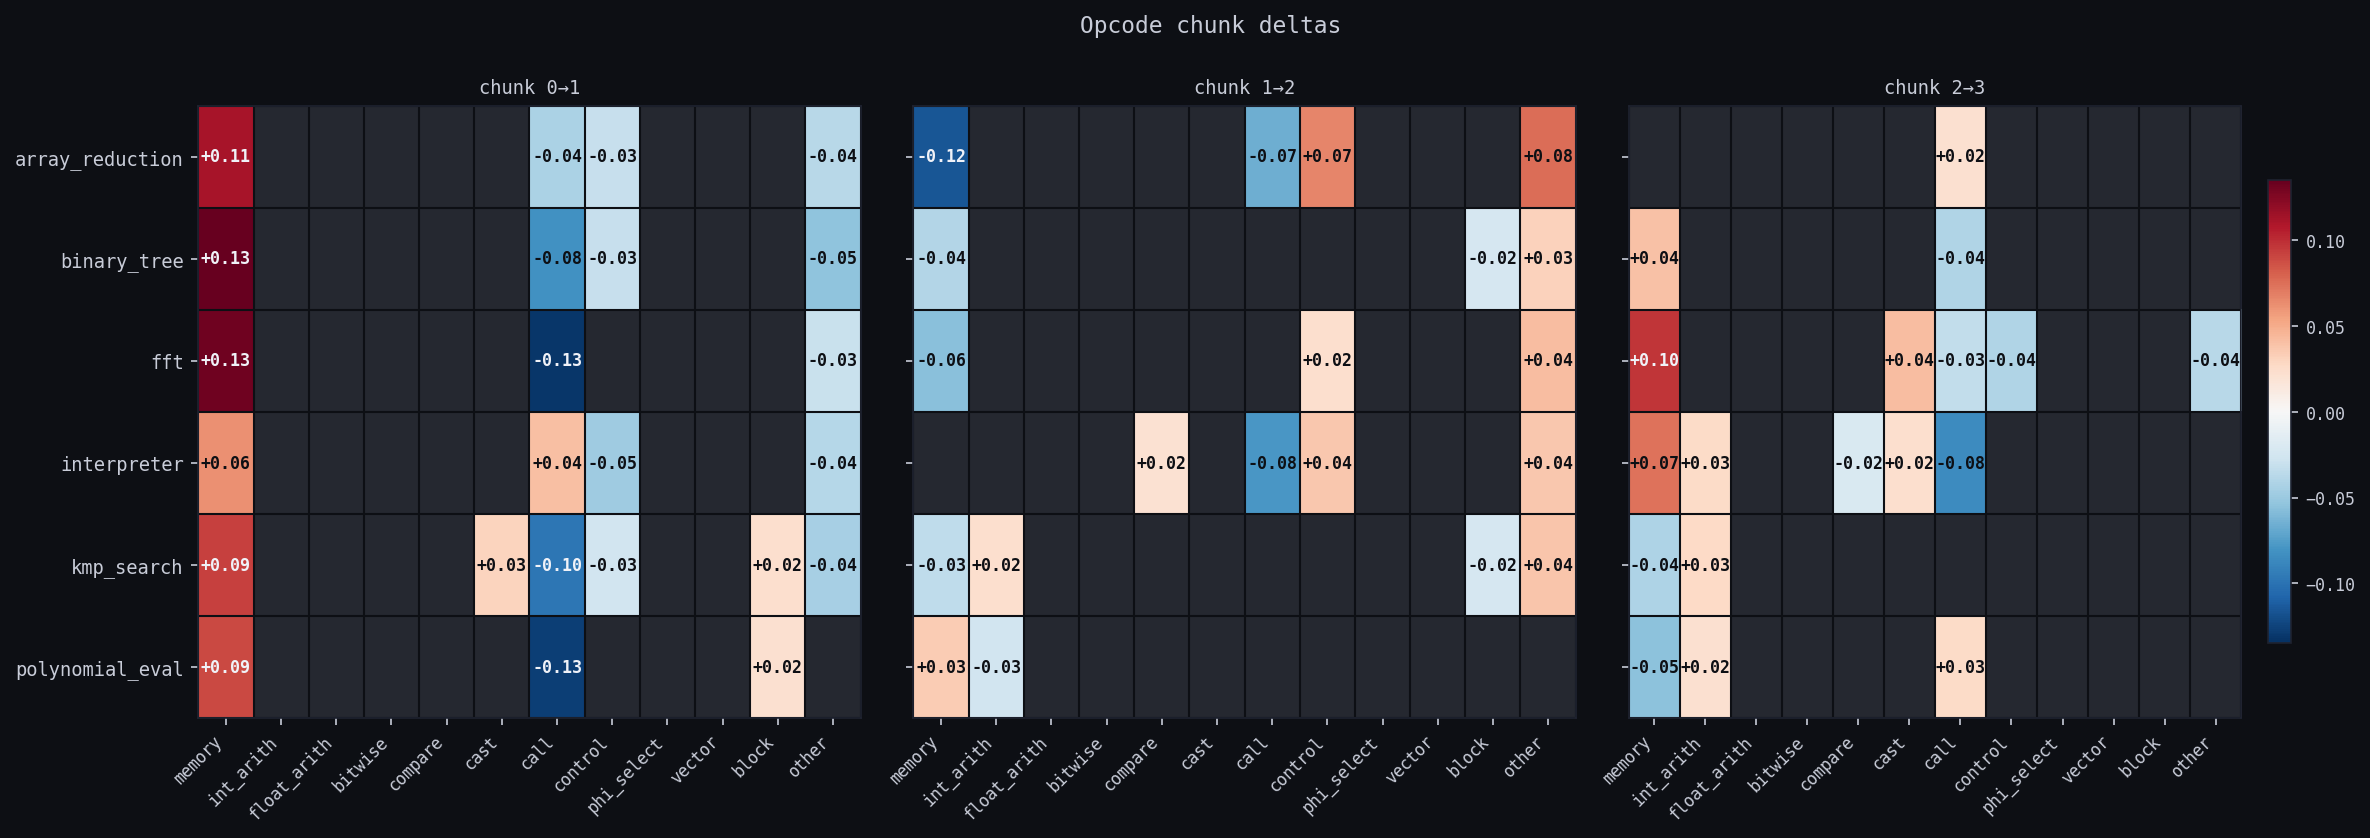
\includegraphics[width=\columnwidth]{features_op.png}
  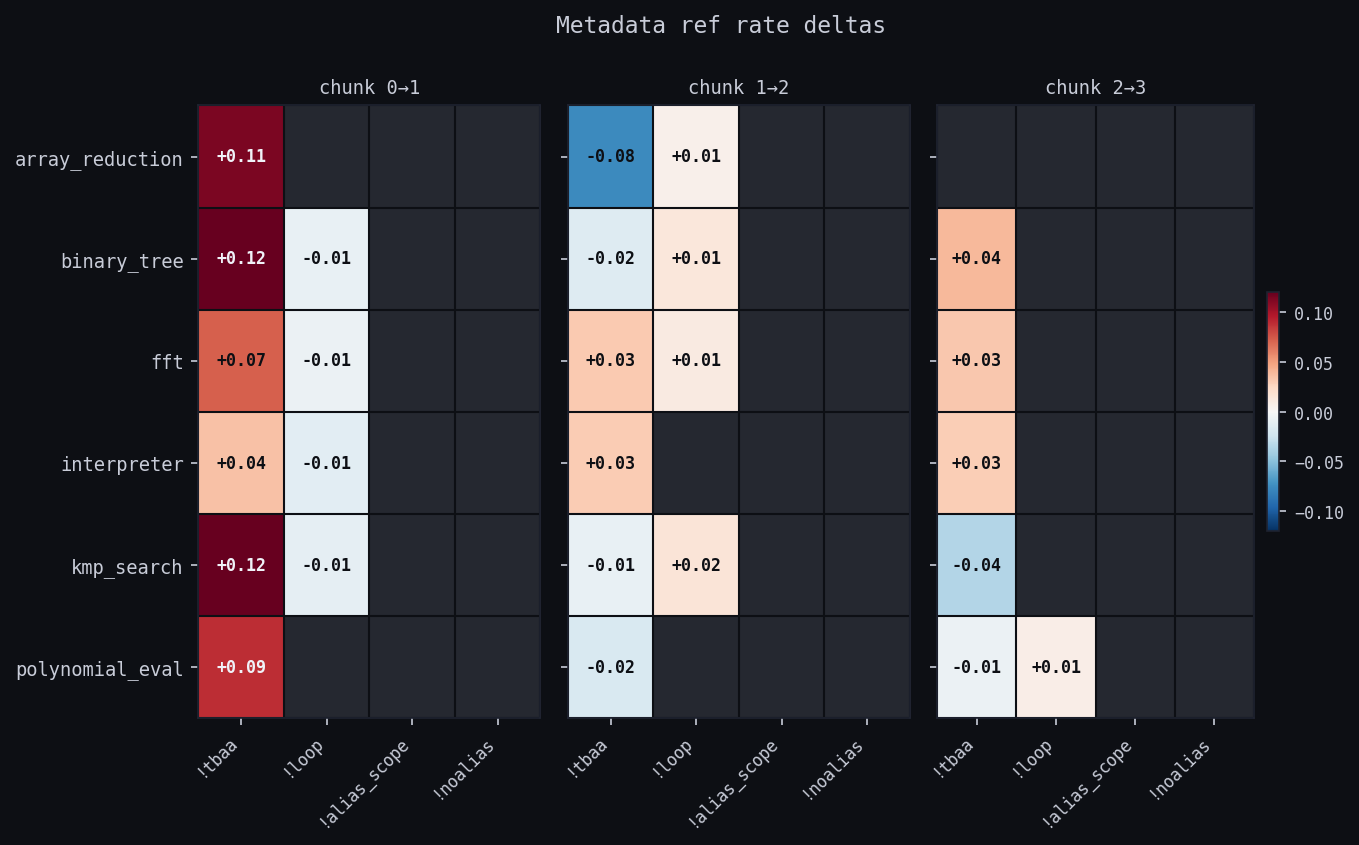
\includegraphics[width=\columnwidth]{features_meta.png}
  \caption{Chunk-to-chunk deltas for the six training functions.
           \emph{Top}: opcode-category frequencies (12 categories).
           \emph{Bottom}: metadata-reference rates (\texttt{tbaa},
           \texttt{llvm.loop}, \texttt{alias.scope}, \texttt{noalias}).
           Functions with rich loop structure (\texttt{fft},
           \texttt{kmp\_search}) show large deltas in memory and control
           categories, distinguishing them from straight-line functions.}
  \label{fig:features}
\end{figure}

\subsection{Benchmark Selection and Baseline Landscape}
\label{sec:baseline}
From the 38-function pool, six benchmarks were selected for the RL training
phase based on three criteria from the EDA: (1) at least one random sequence
achieves lower execution time than \opt{3}, confirming the pass menu is
expressive enough for that function; (2) a high coefficient of variation
(CV) across random sequences, indicating a rugged optimisation landscape
with strong reward gradient for learning; and (3) diversity of computational
profile (call-heavy, arithmetic-heavy, loop/vectorize, pointer/struct).

Figure~\ref{fig:ceiling} shows the best random-search result versus baselines
for all 38 pool functions, used to identify which functions satisfy criterion
(1).
Table~\ref{tab:baselines} shows the key statistics for the selected six.

\begin{figure}[t]
  \centering
  \includegraphics[width=\columnwidth]{ceiling_gaps.png}
  \caption{Best random-search result vs.\ \opt{3} across all 38 pool
           functions (25{,}000 sequences each).
           Functions to the left of zero have at least one random sequence
           that beats \opt{3}, confirming the pass menu is expressive for
           that function.  The six training benchmarks
           (\texttt{interpreter}, \texttt{kmp\_search},
           \texttt{polynomial\_eval}, \texttt{fft},
           \texttt{array\_reduction}, \texttt{binary\_tree}) appear in the
           top tier and satisfy all three selection criteria.}
  \label{fig:ceiling}
\end{figure}

\begin{table}[t]
\caption{Six training benchmarks: \opt{3} baseline, best random-search
result, and CV across 25{,}000 random sequences.
``vs O3'' is percentage improvement (negative = faster than \opt{3}).}
\label{tab:baselines}
\centering
\begin{tabular}{lrrrr}
\toprule
Benchmark & O3 (ns) & Best (ns) & vs O3 & CV \\
\midrule
interpreter      &  37{,}918 &  27{,}591 & $-27.2\%$ & 13.9\% \\
kmp\_search      & 886{,}408 & 671{,}195 & $-24.3\%$ & 42.7\% \\
polynomial\_eval & 417{,}235 & 364{,}235 & $-12.7\%$ & 46.0\% \\
fft              &  46{,}509 &  41{,}852 & $-10.0\%$ & 35.5\% \\
array\_reduction &  97{,}184 &  92{,}619 &  $-4.7\%$ & 36.6\% \\
binary\_tree     & 117{,}990 & 107{,}087 &  $-9.2\%$ & 18.4\% \\
\bottomrule
\end{tabular}
\end{table}

\subsection{Pass Impact Analysis}
The EDA quantified per-pass marginal impact using two metrics.
\emph{Top-decile enrichment} is the ratio of a pass's presence rate in the
top 10\% of sequences to its overall presence rate ($\approx$30\% under
uniform sampling with a 20-pass budget).
\emph{Geometric-mean speedup} compares sequences containing a pass against
matched sequences not containing it.
\pass{inline} is the most impactful pass by both metrics
(enrichment $2.35\times$, geo-mean speedup $1.26\times$), consistent with
its role as a \emph{pass enabler}: eliminating call overhead exposes callee
bodies to constant propagation, dead-code elimination, and loop
transformations.
\pass{simplifycfg}, \pass{sroa}, and \pass{mem2reg} rank second through
fourth, confirming that SSA promotion and CFG cleanup are prerequisites for
most downstream analyses.

\subsection{Sequence Length Analysis}
\label{sec:seqlen}
Sequences are sampled with lengths uniformly distributed across 1--20,
reflecting the uniform sampling strategy.
Figure~\ref{fig:seqlen} shows the best-found sequence length per benchmark
grouped by difficulty tier.
Medians range from 16 to 18 passes across all tiers with no systematic
spike at the 20-pass cap, validating $K = 20$ as the horizon and confirming
that optimal sequences do not require the full budget---the \pass{Stop}
action is available but the distribution of best lengths shows that 17--18
passes captures most of the achievable gain.

\begin{figure}[t]
  \centering
  \includegraphics[width=\columnwidth]{seq_length_by_tier.png}
  \caption{Best-found sequence length per benchmark, grouped by difficulty
           tier across all 38 pool functions.
           Medians are 18 (beats-O3), 17 (reachable), 18 (gap), 16 (hard).
           No tier spikes at the 20-pass cap, supporting $K = 20$ as the
           horizon and the \pass{Stop} token as an available but
           non-mandatory early-exit.}
  \label{fig:seqlen}
\end{figure}

% ─────────────────────────────────────────────────────────────────────────────
\section{Methodology}

\subsection{Policy Architecture}
\label{sec:arch}
We train two autoregressive policy architectures.
Both observe the \emph{current} IR feature vector $\mathbf{f}_t$ (updated
after applying the previous pass) alongside the history of actions taken so
far, enabling the policy to condition each choice on what the previous passes
actually did to the IR.

\paragraph{Auto-GRU.}
\texttt{Auto-GRU} (\texttt{src/ppo/model/auto\_gru.rs}) maintains a recurrent
hidden state updated at each step.
The initial hidden state is seeded from $\mathbf{f}_0$ projected to the GRU
dimension; subsequent updates receive the concatenation of the current IR
features and the one-hot action embedding.
The policy and value heads read from the final hidden state.
The recurrent inductive bias naturally gives recent IR state more influence
than earlier steps, which aligns with the observation that late-stage passes
see the most refined IR.

\paragraph{Auto-TFX.}
\texttt{Auto-TFX} (\texttt{src/ppo/model/auto\_tfx.rs}) builds an explicit
token sequence and applies a transformer encoder:
%
\begin{equation}
\mathbf{s}_t = \bigl[W_{\text{ir}}\,\mathbf{f}_t \;\big|\;
               E[a_0], \ldots, E[a_{t-1}]\bigr]
               \in \mathbb{R}^{(1+t)\times d}
\label{eq:tokens}
\end{equation}
%
where $W_{\text{ir}} \in \mathbb{R}^{48 \times d}$ projects the current IR
features (\texttt{ir\_proj}) and $E \in \mathbb{R}^{29 \times d}$
is a learned action embedding table (\texttt{action\_embed}).
No causal mask is applied: since we decode one step at a time, the full
sequence is always available and unrestricted cross-step attention is
beneficial.
The \textbf{policy head} reads from the last token (position $t$) to produce
logits over 29 actions; the \textbf{value head} reads from token 0 (the
current IR projection) to estimate $V(\mathbf{f}_t)$.

The two architectures represent complementary computational hypotheses.
Auto-GRU's implicit memory introduces a recency bias that may help when the
relevant IR context is recent; Auto-TFX's explicit attention can directly
compare any step's IR state against any prior action, which may help when
pass interactions are non-local.

\paragraph{Batched replay.}
During PPO updates, recomputing all logits naively requires one forward per
step per episode ($N \times K$ calls).
\texttt{replay\_batch} (\texttt{auto\_tfx.rs:191}) reduces this to $K$
batched calls by iterating over step positions: at step $t$, all episodes
with length $> t$ are stacked into a single batch of shape
$[|\text{active}|,\,1{+}t,\,d]$ and processed together.
Episodes shorter than $t$ are absent, requiring no padding mask.
Each step is assigned weight $w = 1/(N_{\text{chunk}} \cdot K_i)$ in the
loss, averaging first within episodes then across them
(\texttt{ppo/mod.rs}).

\subsection{PPO Training}
\label{sec:ppo}

PPO is an on-policy algorithm structured as a collection--update loop.
At each epoch, the current policy rolls out a batch of complete episodes
under its current parameters; those episodes---each a sequence of
(state, action, log-prob, return) tuples---form the training batch for
that round.
The policy parameters are then updated via multiple gradient steps over
the batch before the next collection round begins.
The core challenge is that these gradient steps move the policy away from
the distribution under which the data was collected, making the stored
log-probabilities increasingly stale.
The clipped surrogate objective bounds how far the updated policy can
deviate from the collection policy, keeping gradient estimates valid while
still extracting multiple updates from each batch.

\paragraph{Policy gradient objective.}
At each PPO update we have a mini-batch of episodes with stored
(state, action, log-prob, return, advantage) tuples.
For each step $t$ we compute the probability ratio
$\rho_t = \pi_\theta(a_t | s_t) / \pi_{\theta_{\text{old}}}(a_t | s_t)$
and form the clipped surrogate:
%
\begin{equation}
L^{\text{CLIP}}_t = \min\!\bigl(
  \rho_t \hat{A}_t,\;
  \text{clip}(\rho_t, 1{-}\epsilon, 1{+}\epsilon)\,\hat{A}_t
\bigr)
\label{eq:ppo}
\end{equation}
%
with clip threshold $\epsilon = 0.2$.
The total loss is:
%
\begin{equation}
L = -\mathbb{E}_t\!\left[L^{\text{CLIP}}_t\right]
    + c_v\,\mathbb{E}_t\!\left[(V_\theta(s_t) - R_t)^2\right]
    - c_e\,\mathbb{E}_t\!\left[H(\pi_\theta(\cdot|s_t))\right]
\label{eq:ppofull}
\end{equation}
%
where $c_v = 0.5$ is the value coefficient, $c_e = 0.03$ is the entropy
bonus coefficient, and $H$ is Shannon entropy encouraging exploration.
A per-minibatch KL early-stop threshold of 0.05 aborts remaining inner
epochs when the policy update is too large, preventing entropy collapse
(\texttt{ppo/mod.rs}).

\paragraph{Episode collection.}
Before any training begins, serial baselines (\opt{0}--\opt{3}) are
collected for each function under stable single-threaded conditions.
Episode collection during training is parallelised across all available
CPU cores using Rayon.
Section~\ref{sec:benchnoise} describes how we characterised and accounted
for the timing overhead this introduces.

\subsection{Benchmark Noise Characterisation}
\label{sec:benchnoise}
Because episode rewards are runtime measurements, systematic timing bias
from parallel execution would corrupt the reward signal.
The \texttt{bench-noise} command measures this bias: for each benchmark
binary it records the solo execution time, then runs the same binary
simultaneously across 16 Rayon workers and records the distribution of
measurements.

\begin{figure}[t]
  \centering
  \includegraphics[width=0.48\columnwidth]{bench_noise-fft.png}
  \hfill
  \includegraphics[width=0.48\columnwidth]{bench_noise-kmp.png}
  \caption{Timing distributions under solo vs.\ 16-worker parallel
           execution for \texttt{fft} (left) and \texttt{kmp\_search}
           (right).  Parallel overhead is small and consistent across
           all six benchmarks.}
  \label{fig:benchnoise}
\end{figure}

Parallel overhead was small and consistent across all six benchmarks.
We account for it by applying a fixed noise margin that pessimises the
\opt{3} baseline when computing episode rewards during training
(\texttt{PARALLEL\_NOISE\_MARGIN = 1.01}, \texttt{src/llvm/benchmark.rs}).
This ensures that a policy sequence must beat \opt{3} by more than the
measurement noise floor to receive a positive reward.
Final evaluation uses serial benchmarking only.

\subsection{Return Formulations}
\label{sec:returns}
The terminal reward---a single real benchmark measurement per episode---is
the ground-truth signal for the optimisation objective.
The central challenge is credit assignment: which of the $K$ actions in a
sequence contributed to the final outcome?
We analyse two principled formulations and include an IR-step ablation.

Where per-step shaping is applied, a step is classified as a no-op when the
normalised instruction-count delta $|\Delta I_t| < 0.01$ \emph{and} the L1
distance between IR feature vectors before and after is below $0.05$
(\texttt{src/ppo/noop.rs}).
The dual threshold is necessary because passes such as \pass{loop-rotate}
and \pass{licm} restructure loop metadata without changing instruction count.

\paragraph{Episode return.}
The episode return assigns the terminal speedup $r$ uniformly to every
step (\texttt{src/ppo/returns/episode\_return.rs}):
$R_t = r \;\forall\, t$.
This is the unbiased maximum-likelihood estimate: the only externally
measured quantity is $r$, and distributing it equally makes no assumptions
about which steps were responsible.
All shaping alternatives introduce a bias in exchange for reduced variance;
episode return provides the baseline against which that trade-off is measured.
The training challenge with episode return is that when $r < 0$---as it is
for most sequences early in training---every action is penalised equally,
including actions that would have been beneficial with a different
continuation.
The value head must learn to disentangle this noise from the policy gradient
signal.

\paragraph{Instruction-weighted terminal return.}
Episode return assigns the same terminal reward to every step, so a pass
that substantially reduces instruction count receives the same gradient
signal as an immediately following no-op.
The instruction-weighted formulation
(\texttt{src/ppo/returns/weighted.rs}) breaks this
symmetry without introducing any signal not already present in the IR:
each step's return is scaled by its share of the total instruction
reduction, steps that reduced instructions earn a small direction bonus,
and steps that meet both no-op thresholds are penalised:
%
\begin{equation}
R_t = r \cdot \frac{|\Delta I_t|}{\sum_s |\Delta I_s|}
      + \delta \cdot \operatorname{sign}(-\Delta I_t)
      - p \cdot \mathbf{1}[\text{noop}_t]
\label{eq:weightedreturn}
\end{equation}
%
where $\Delta I_t$ is the normalised instruction-count change at step $t$
(\texttt{src/llvm/ir.rs}, \texttt{step\_delta()}),
$\delta = 0.05$ is the direction bonus, and $p = 0.025$ is the no-op
penalty.
The key property is that the sum of the first term over all steps equals $r$:
the terminal speedup is preserved, only its distribution across steps is
changed.
This gives the value head more informative per-step targets while keeping
the overall objective identical to episode return.

\paragraph{IR-step return (ablation).}
The \texttt{ir-step} formulation
(\texttt{src/ppo/returns/ir\_step\_return.rs}) uses the per-step IR
instruction-count delta as the reward, bypassing benchmarking entirely
(\texttt{--skip-benchmark}).
This decouples the policy architecture and training loop from the runtime
reward signal, providing a fast verification that the model can learn a
well-defined dense objective.
IR count reduction is not our optimisation target; this configuration
is not evaluated as a policy and its training results are interpreted
only as an infrastructure check.

\subsection{Advantage Estimation}
\label{sec:advantages}
The return $R_t$ is not used directly in the PPO objective; the
\emph{advantage} $\hat{A}_t$ subtracts a baseline to reduce variance.
We use the standard learned value baseline
(\texttt{src/ppo/advantages/baseline.rs}):
$\hat{A}_t = R_t - V_\theta(\mathbf{f}_t)$.
The resulting advantages are batch-normalised (zero mean, unit variance)
across all steps in the mini-batch, ensuring roughly half of actions are
reinforced and half penalised regardless of the absolute reward scale.

The quality of this estimator is measured by explained variance:
%
\begin{equation}
\text{EV} = 1 - \frac{\operatorname{Var}(R_t - V_\theta)}{\operatorname{Var}(R_t)}
\label{eq:ev}
\end{equation}
%
EV near 1 indicates the value head is accurately predicting returns,
providing a tightly calibrated baseline.
EV near 0 or negative indicates the value head is not tracking returns and
the baseline is adding noise rather than removing it.
In our episode-return runs the value head's EV reaches $0.69$ (Auto-TFX)
and $0.59$ (Auto-GRU) by epoch 100 (Section~\ref{sec:results}), confirming
that the 48-dimensional IR state representation---augmented with action
history---is sufficient for both architectures to learn a useful value function.
This is a non-trivial result: with sparse terminal rewards and high-variance
episode outcomes, value learning is often the bottleneck in on-policy methods.

\subsection{Training Setup}
All experiments train for 100 epochs.
Each epoch collects 256 episodes in parallel, then runs 4 PPO inner epochs
on mini-batches of 128 episodes.
The optimiser is AdamW with a cosine learning-rate schedule from $10^{-3}$
to $\approx 0$ over 100 epochs.
The training framework is Rust + Burn~\cite{burn} on the \texttt{wgpu}
backend.

Table~\ref{tab:hparams} lists all model and training hyperparameters.
Architecture parameters are persisted in \texttt{arch\_config.json} at
checkpoint save time and loaded automatically; training parameters are set
via command-line flags (\texttt{src/config.rs}).

\begin{table}[t]
\caption{Model and training hyperparameters for all reported runs.
Weighted-return parameters apply only when \texttt{--returns weighted}.
\texttt{--value-coef} defaults to 0.5 and can be adjusted per run.}
\label{tab:hparams}
\centering
\begin{tabular}{ll}
\toprule
Parameter & Value \\
\midrule
\multicolumn{2}{l}{\emph{Model}} \\
$d_{\text{model}}$ & 128 \\
Transformer layers & 2 \\
Attention heads & 4 \\
Feed-forward width & 256 \\
Dropout & 0.1 \\
Head hidden dim & 64 \\
IR chunks & 4 $\to$ 48-dim feature \\
Actions & 29 (28 passes + Stop) \\
Horizon $K$ & 20 \\
\midrule
\multicolumn{2}{l}{\emph{Training}} \\
Epochs & 100 \\
Episodes / epoch & 256 \\
PPO inner epochs & 4 \\
Mini-batch size & 128 \\
KL early-stop & 0.05 \\
Learning rate & $10^{-3}$ cosine \\
Clip $\epsilon$ & 0.2 \\
Entropy coef $c_e$ & 0.03 \\
Value coef $c_v$ & 0.5 \\
No-op $\tau_{\text{count}}$ & 0.01 \\
No-op $\tau_{\text{feat}}$ & 0.05 \\
No-op penalty $p$ & 0.025 (weighted) \\
Direction bonus $\delta$ & 0.05 (weighted) \\
Noise margin & 1.01 \\
\bottomrule
\end{tabular}
\end{table}

\subsection{Reproducibility Verification}
\label{sec:diagnose}
Training caches the top-performing sequences observed during episode
collection (\texttt{src/llvm/top\_sequences.rs}).
The \texttt{diagnose} command re-benchmarks these sequences serially under
controlled conditions to verify that the cached speedups are reproducible
rather than artefacts of parallel timing noise.
Each sequence is benchmarked 20 times independently to obtain a mean,
standard deviation, and full distribution.

\begin{figure}[t]
  \centering
  \includegraphics[width=\columnwidth]{diagnose.png}
  \caption{Diagnose results for top sequences from the episode-return run.
           Left: mean speedup (bar, $\pm$1 std) vs.\ cached training speedup
           (dot).  Right top: scatter of cached vs.\ measured speedup
           showing strong correlation.  Right bottom: per-sequence speedup
           distributions across 20 re-runs, confirming low variance.
           The dominant sequences are from \texttt{interpreter} and
           \texttt{kmp\_search}, consistent with their high
           random-search ceiling.}
  \label{fig:diagnose}
\end{figure}

Figure~\ref{fig:diagnose} shows that cached training speedups correlate
strongly with re-measured values, and that the per-sequence distributions
are tight, confirming the reward signal is reproducible and not dominated
by timing noise.

% ─────────────────────────────────────────────────────────────────────────────
\section{Training Results}
\label{sec:results}

\subsection{Episode Return}
\label{sec:results-episode}

\begin{figure}[t]
  \centering
  \includegraphics[width=\columnwidth]{auto-tfx-episode.png}
  \caption{Training diagnostics for Auto-TFX with episode return
           (100 epochs, 256 episodes/epoch).
           Mean episode speedup and EMA rise from $-0.40$ to $+0.091$;
           per-function curves show \texttt{interpreter} and
           \texttt{kmp\_search} leading.
           Entropy decays as the policy concentrates.
           Explained variance reaches $0.69$.
           No-op rate stabilises near 30\%.}
  \label{fig:training-tfx-episode}
\end{figure}

Figure~\ref{fig:training-tfx-episode} shows Auto-TFX training under episode
return.
Mean episode speedup climbs steadily from $-0.40$ to $+0.091$ at epoch 100,
with the EMA reaching $+0.080$.
Explained variance rises from near-zero to $0.69$ by epoch 100.
This steady improvement confirms that the 48-dimensional delta representation
encodes sufficient signal for the transformer to learn a useful value function
and make progressively better pass selections.

Entropy declines monotonically from near-maximum to roughly 30\% of maximum,
reflecting progressive policy concentration without collapse.
The no-op percentage stabilises near 30\%, showing the policy selectively
avoids structurally neutral passes while continuing to exploit the full horizon.

\begin{figure}[t]
  \centering
  \includegraphics[width=\columnwidth]{auto-gru-episode.png}
  \caption{Training diagnostics for Auto-GRU with episode return
           (100 epochs, 256 episodes/epoch).
           Mean episode speedup rises from $-0.44$ to $+0.043$; explained
           variance reaches $0.59$. Convergence is slower and final speedup
           lower than Auto-TFX, consistent with the GRU's weaker capacity
           for long-range pass interactions.}
  \label{fig:training-gru-episode}
\end{figure}

Auto-GRU training under episode return follows the same qualitative
trajectory as Auto-TFX but converges more slowly
(Figure~\ref{fig:training-gru-episode}).
Mean episode speedup rises from $-0.44$ at epoch 0 to $+0.043$ at epoch 100,
with explained variance reaching $0.59$.
The slower rise in both speedup and EV compared to Auto-TFX suggests that
the transformer's explicit attention over all prior steps provides a material
advantage for this task.
Quantitative evaluation results are presented in Section~\ref{sec:arch-comparison}.

\subsection{Instruction-Weighted Return}
\label{sec:results-weighted}

\begin{figure}[t]
  \centering
  \includegraphics[width=\columnwidth]{auto-tfx-weighted.png}
  \caption{Training diagnostics for Auto-TFX with instruction-weighted
           return (100 epochs, 256 episodes/epoch).
           Mean episode speedup reaches only $+0.012$ at epoch 100
           despite explained variance of $0.87$---higher than the episode
           runs---reflecting that the value head learned per-step IR targets
           accurately but those targets are a poor proxy for runtime speedup.
           No-op percentage stabilises near 41\%, above the 30\% seen under
           episode return.}
  \label{fig:training-tfx-weighted}
\end{figure}

\begin{figure}[t]
  \centering
  \includegraphics[width=\columnwidth]{auto-gru-weighted.png}
  \caption{Training diagnostics for Auto-GRU with instruction-weighted
           return (100 epochs, 256 episodes/epoch).
           Final mean episode speedup is $+0.023$; explained variance
           reaches $0.86$.  Pattern mirrors Auto-TFX weighted: high EV,
           low actual speedup, elevated no-op rate.}
  \label{fig:training-gru-weighted}
\end{figure}

Figures~\ref{fig:training-tfx-weighted} and \ref{fig:training-gru-weighted}
show training under the instruction-weighted return for Auto-TFX and Auto-GRU
respectively.
Both runs exhibit a distinctive pattern: explained variance climbs higher than
the corresponding episode runs ($0.87$ and $0.86$ vs.\ $0.69$ and $0.59$),
yet mean episode speedup at the end of training is dramatically lower
($+0.012$ and $+0.023$ vs.\ $+0.091$ and $+0.043$).

The high EV confirms that the value head has learned accurate per-step
return predictions---the shaped targets are well-behaved and predictable.
The low speedup reveals that the objective the policy actually optimised
diverged from runtime improvement.
The instruction-weighted formulation rewards each step in proportion to its
share of total IR-instruction reduction; a pass that aggressively reduces
IR count receives a large positive return regardless of whether the resulting
binary runs faster.
With no direct incentive to maintain runtime speedup, the policy converges
toward IR-compressing sequences that do not translate to wallclock gains.

Per-function evaluation results for both weighted runs are in
Tables~\ref{tab:eval-tfx-weighted} and \ref{tab:eval-gru-weighted}
(Section~\ref{sec:arch-comparison}).
Mean greedy speedup across the six functions is $+0.065$ (6.5\%) for
Auto-TFX and $+0.092$ (9.2\%) for Auto-GRU---lower than the corresponding
episode runs in both cases.
Notably, \texttt{array\_reduction} regresses to greedy below \opt{3} for
both weighted architectures, whereas episode return keeps it positive.

\subsection{Architecture Comparison}
\label{sec:arch-comparison}

Table~\ref{tab:arch-comparison} summarises mean greedy evaluation speedup and
final value-head explained variance for all four configurations.

\begin{table}[t]
\caption{Evaluation summary: mean greedy speedup across six functions and
final explained variance (epoch 100) for each configuration.
Speedup is the mean of per-function greedy speedups relative to \opt{3}.}
\label{tab:arch-comparison}
\centering
\begin{tabular}{llrr}
\toprule
Architecture & Return & Greedy mean & EV \\
\midrule
Auto-TFX & Episode  & $+0.104$ & $0.69$ \\
Auto-GRU & Episode  & $+0.114$ & $0.59$ \\
Auto-TFX & Weighted & $+0.065$ & $0.87$ \\
Auto-GRU & Weighted & $+0.092$ & $0.86$ \\
\bottomrule
\end{tabular}
\end{table}

Both architectures achieve higher greedy evaluation speedup under episode
return than under instruction-weighted return.
The return-formulation effect is consistent across architectures: weighted
return reduces mean greedy speedup by 37\% for Auto-TFX and 19\% for Auto-GRU.
Explained variance is higher for weighted runs ($0.87$/$0.86$ vs.\
$0.69$/$0.59$), confirming that the per-step IR targets are easier to predict
than sparse terminal speedup---but this accuracy advantage does not translate
to better runtime performance.

On the architecture dimension, Auto-GRU slightly outperforms Auto-TFX under
both return formulations in greedy evaluation despite showing lower mean
speedup during training.
This arises because the reported evaluation uses the best checkpoint saved
during training (rather than the final epoch), and an early peak epoch can
produce a well-calibrated greedy sequence even if the final policy has
overfitted or explored away from it.
Within each return formulation the two architectures are broadly comparable,
suggesting that neither the recurrent nor the attention-based memory has a
decisive advantage at this problem scale.

% ─────────────────────────────────────────────────────────────────────────────
\section{Policy Evaluation}

\subsection{Evaluation Protocol}
\label{sec:eval-protocol}
The trained policy is evaluated on the six training functions.
All evaluation runs use serial benchmarking: 5 runs of 200 iterations each
for the policy sequences, and 3 runs of 200 iterations for the baselines.
We compare four strategies against the \opt{3} reference:
\begin{itemize}
  \item \textbf{Random mean / best}: mean and best speedup across 20
        uniformly sampled sequences of length up to $K$.
  \item \textbf{Greedy}: deterministic argmax decoding.
  \item \textbf{Sample best}: best of 20 stochastic policy rollouts.
\end{itemize}

\subsection{Episode Return Evaluation}

\begin{table}[t]
\caption{Evaluation speedup relative to \opt{3} for Auto-TFX trained with
episode return. Positive = faster than \opt{3}.}
\label{tab:eval-tfx-episode}
\centering
\setlength{\tabcolsep}{4pt}
\begin{tabular}{lrrrr}
\toprule
Function & rand mean & rand best & greedy & samp best \\
\midrule
array\_reduction & $-0.795$ & $-0.039$ & $+0.075$ & $+0.095$ \\
binary\_tree     & $-0.089$ & $+0.062$ & $+0.027$ & $+0.066$ \\
fft              & $-0.547$ & $-0.033$ & $-0.016$ & $+0.037$ \\
interpreter      & $-0.252$ & $+0.010$ & $+0.271$ & $+0.276$ \\
kmp\_search      & $-0.101$ & $+0.209$ & $+0.237$ & $+0.278$ \\
polynomial\_eval & $-0.261$ & $+0.120$ & $+0.031$ & $+0.149$ \\
\bottomrule
\end{tabular}
\end{table}

\begin{figure}[t]
  \centering
  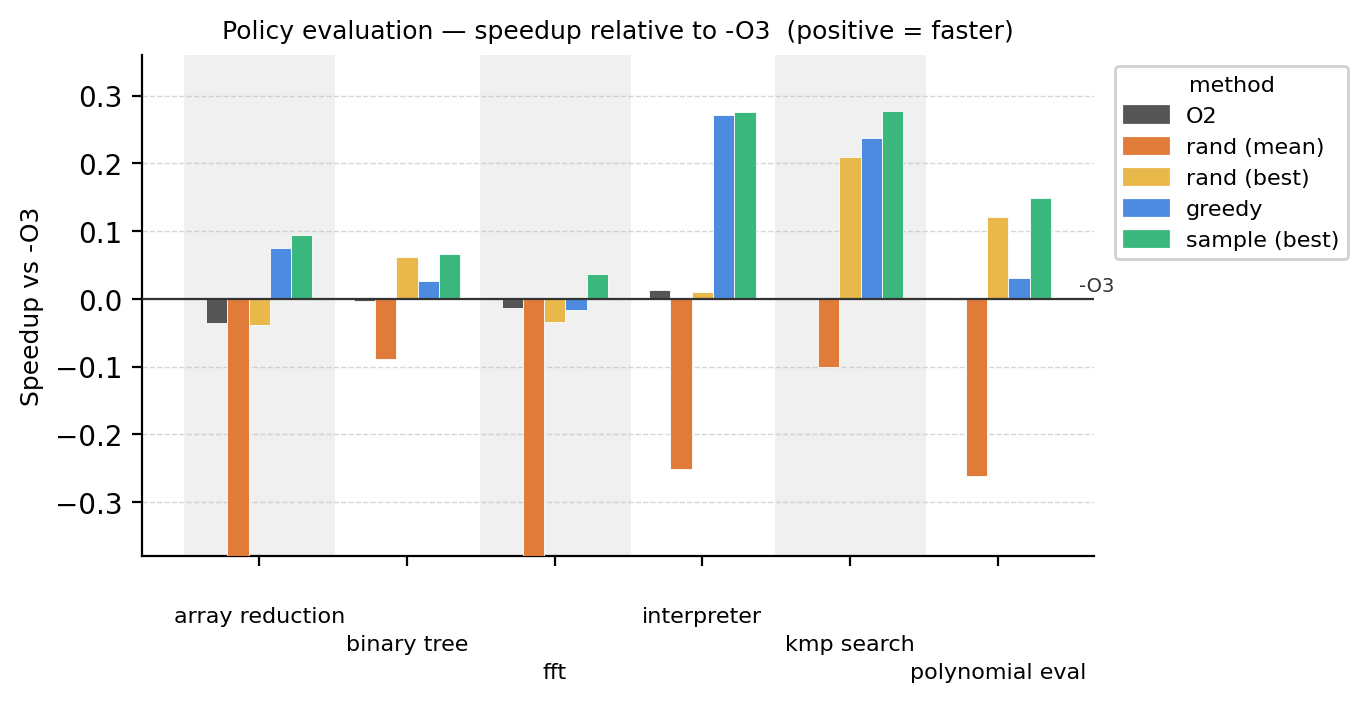
\includegraphics[width=\columnwidth]{eval.png}
  \caption{Evaluation speedup for Auto-TFX with episode return.
           Greedy decoding beats \opt{3} on five of six functions;
           stochastic sample-best extends this to all six.
           Random mean is strongly negative on
           \texttt{array\_reduction} and \texttt{fft}, confirming these
           functions require a learned policy rather than lucky search.}
  \label{fig:eval-tfx-episode}
\end{figure}

Table~\ref{tab:eval-tfx-episode} and Figure~\ref{fig:eval-tfx-episode}
show evaluation results for Auto-TFX with episode return.
Greedy decoding beats \opt{3} on five of six functions (all except
\texttt{fft}, where the greedy sequence is marginally slower at $-0.016$).
Mean greedy speedup is $+0.104$ (10.4\%).
\texttt{interpreter} and \texttt{kmp\_search} show the largest gains
(27.1\% and 23.7\%), while \texttt{fft} is the only function where greedy
fails to beat the baseline.
Stochastic sampling (best of 20) recovers \texttt{fft} to $+0.037$ and
extends all other functions, beating \opt{3} on all six.

The random-mean baseline is strongly negative on \texttt{array\_reduction}
($-0.79$) and \texttt{fft} ($-0.55$), confirming that most random sequences
are harmful on these functions and that a learned policy is required.
Greedy decoding outperforms the best of 20 random sequences on four of six
functions, demonstrating that the policy has learned more than identifying the
easiest sequences in the landscape.

\begin{table}[t]
\caption{Evaluation speedup relative to \opt{3} for Auto-GRU trained with
episode return. Positive = faster than \opt{3}.}
\label{tab:eval-gru-episode}
\centering
\setlength{\tabcolsep}{4pt}
\begin{tabular}{lrrrr}
\toprule
Function & rand mean & rand best & greedy & samp best \\
\midrule
array\_reduction & $-1.014$ & $-0.036$ & $+0.088$ & $+0.097$ \\
binary\_tree     & $-0.139$ & $+0.086$ & $+0.022$ & $+0.092$ \\
fft              & $-0.593$ & $+0.050$ & $+0.003$ & $+0.031$ \\
interpreter      & $-0.217$ & $+0.268$ & $+0.207$ & $+0.281$ \\
kmp\_search      & $-0.020$ & $+0.223$ & $+0.236$ & $+0.267$ \\
polynomial\_eval & $-0.286$ & $+0.104$ & $+0.127$ & $+0.159$ \\
\bottomrule
\end{tabular}
\end{table}

\subsection{Instruction-Weighted Return Evaluation}

Tables~\ref{tab:eval-tfx-weighted} and \ref{tab:eval-gru-weighted} show
evaluation results for Auto-TFX and Auto-GRU trained with instruction-weighted
return.
Both architectures achieve lower mean greedy speedup than their episode-return
counterparts: $+0.065$ (TFX) and $+0.092$ (GRU) vs.\ $+0.104$ and $+0.114$
under episode return.
\texttt{array\_reduction} regresses below \opt{3} under greedy decoding for
both weighted models, a function that remained positive under episode return.

The two weighted architectures are close to each other in absolute performance,
with Auto-GRU slightly ahead on mean greedy speedup despite its lower training
convergence.
This mirrors the episode-return result and suggests the architecture gap is
small relative to the return-formulation gap.
The dominant function in both weighted evaluations is again
\texttt{interpreter}, where the greedy speedup ($+0.307$/$+0.306$) matches
or exceeds the episode-return results---indicating that \texttt{interpreter}'s
optimisation landscape is robust to return formulation, likely because it
offers large, clear gains that any positive signal can find.

\begin{table}[t]
\caption{Evaluation speedup relative to \opt{3} for Auto-TFX trained with
instruction-weighted return. Positive = faster than \opt{3}.}
\label{tab:eval-tfx-weighted}
\centering
\setlength{\tabcolsep}{4pt}
\begin{tabular}{lrrrr}
\toprule
Function & rand mean & rand best & greedy & samp best \\
\midrule
array\_reduction & $-0.814$ & $+0.018$ & $-0.081$ & $-0.053$ \\
binary\_tree     & $-0.139$ & $+0.078$ & $+0.079$ & $+0.081$ \\
fft              & $-0.528$ & $+0.021$ & $+0.008$ & $+0.009$ \\
interpreter      & $-0.229$ & $+0.048$ & $+0.307$ & $+0.308$ \\
kmp\_search      & $-0.097$ & $+0.224$ & $+0.077$ & $+0.081$ \\
polynomial\_eval & $-0.277$ & $+0.155$ & $+0.002$ & $+0.036$ \\
\bottomrule
\end{tabular}
\end{table}

\begin{table}[t]
\caption{Evaluation speedup relative to \opt{3} for Auto-GRU trained with
instruction-weighted return. Positive = faster than \opt{3}.}
\label{tab:eval-gru-weighted}
\centering
\setlength{\tabcolsep}{4pt}
\begin{tabular}{lrrrr}
\toprule
Function & rand mean & rand best & greedy & samp best \\
\midrule
array\_reduction & $-0.896$ & $-0.052$ & $-0.039$ & $-0.011$ \\
binary\_tree     & $-0.058$ & $+0.080$ & $+0.051$ & $+0.058$ \\
fft              & $-0.369$ & $-0.009$ & $+0.016$ & $+0.030$ \\
interpreter      & $-0.202$ & $+0.248$ & $+0.306$ & $+0.306$ \\
kmp\_search      & $-0.044$ & $+0.252$ & $+0.102$ & $+0.107$ \\
polynomial\_eval & $-0.261$ & $+0.129$ & $+0.118$ & $+0.133$ \\
\bottomrule
\end{tabular}
\end{table}

\subsection{Pool-trained Evaluation}
\label{sec:holdout}
To assess whether training on a broader set of functions improves coverage,
we trained an additional Auto-TFX policy with episode return on all 38 pool
functions simultaneously for 100 epochs.
Figure~\ref{fig:eval-fullpool} shows training diagnostics for this run.

\begin{figure}[t]
  \centering
  \includegraphics[width=\columnwidth]{auto-tfx-pool.png}
  \caption{Training diagnostics for Auto-TFX trained on all 38 pool functions
           with episode return.  Mean episode speedup and explained variance
           remain near zero throughout training, indicating the model did not
           converge within 100 epochs.}
  \label{fig:eval-fullpool}
\end{figure}

The pool-trained model failed to converge: mean episode speedup at epoch 100
is $-0.51$ and explained variance is $0.065$, indicating the value head never
learned a useful baseline.
Greedy evaluation across all 38 functions produces negative speedup on every
function (mean $-2.50$).
The likely cause is insufficient episodes per function: each of the 38
functions receives far fewer episodes per epoch than the six training functions
do in the focused setting, starving the gradient of the per-function reward
accumulation needed for convergence.
This result establishes that episodes per function---not total training
epochs---is the binding constraint, and that scaling to a larger pool requires
a proportionally larger per-function episode budget.

% ─────────────────────────────────────────────────────────────────────────────
\section{IR-step Ablation}
\label{sec:ir-ablation}

The \texttt{ir-step} configuration replaces the runtime benchmark reward with
the per-step normalised instruction-count delta, bypassing the benchmarking
pipeline entirely.
This provides a dense, low-noise reward signal that verifies the policy
architecture and PPO loop are functional independently of the sparse runtime
objective.

Training under the IR-step reward converges quickly and reliably:
explained variance reaches $0.986$ by epoch 100 (Figure~\ref{fig:training-irstep}),
far above the episode and weighted runs, confirming that the model is capable
of learning a coherent sequential policy and that the difficulty in the
runtime-reward setting is specific to the sparsity and noise of the real
benchmark measurement.

\begin{figure}[t]
  \centering
  \includegraphics[width=\columnwidth]{auto-tfx-irstep.png}
  \caption{Training diagnostics for Auto-TFX with IR-step return.
           Explained variance approaches 1 rapidly and the mean IR-reduction
           reward reaches $0.56$, confirming the model can learn a dense
           reward reliably.  These results are not compared against runtime
           runs; IR-count reduction is not our optimisation target.}
  \label{fig:training-irstep}
\end{figure}

To quantify the relationship between IR reduction and runtime, we ran the
\texttt{ir-corr} analysis: the top 20 IR-reducing sequences discovered during
IR-step training were re-benchmarked for actual runtime speedup.
Figure~\ref{fig:ircorr} shows the result.

\begin{figure}[t]
  \centering
  \includegraphics[width=\columnwidth]{ir_corr.png}
  \caption{IR instruction-count reduction vs.\ runtime speedup for the
           top 20 sequences from IR-step training (all on \texttt{fft}).
           IR reduction is concentrated in the narrow band 65--67\%
           (a near-vertical cluster), while runtime speedup spans
           $-35\%$ to $-8\%$---uniformly negative.
           High IR reduction does not predict runtime improvement; on
           \texttt{fft} it consistently predicts a slowdown.}
  \label{fig:ircorr}
\end{figure}

All 20 sequences are from \texttt{fft}: the IR-step policy found that
aggressively removing instructions on \texttt{fft} maximises the IR reward,
achieving 65--67\% instruction-count reductions.
Every one of these sequences is slower than \opt{3} at runtime, with speedups
ranging from $-8\%$ to $-35\%$.
The correlation plot is essentially a vertical band: the sequences cluster
tightly in IR reduction (because the policy found a local maximum of that
objective) but span a wide and uniformly negative range of runtime speedup.
This confirms that IR reduction is not a reliable indicator of runtime
improvement---the passes that most aggressively compact the \texttt{fft} IR
also strip away vectorization opportunities and loop structure that the backend
relies on to emit fast machine code.
This result directly motivates the choice of episode return over weighted
return as the primary training signal.

% ─────────────────────────────────────────────────────────────────────────────
\section{Discussion}

\subsection{Return Formulation Analysis}
The episode return is the theoretically cleanest choice for this MDP:
it assigns the observed reward in proportion to each step's prior probability
of being selected, making no assumptions about which steps were causally
responsible.
When a sequence produces a positive terminal speedup, every step that
contributed to reaching that state receives a positive gradient signal---even
steps that performed only modest IR changes.
This is intentional: those steps were part of a winning sequence and did not
hurt, so they should be reinforced.
The cumulative effect is that the policy is steered consistently toward the
class of sequences that produce runtime gains, even if the per-step credit
distribution is imprecise.

The instruction-weighted return redistributes the terminal reward using
per-step IR-instruction reduction as a proxy for contribution.
Despite producing higher explained variance ($0.87$/$0.86$ vs.\
$0.69$/$0.59$)---confirming that the per-step targets are well-behaved and
learnable---both architectures achieved lower evaluation speedup under
weighted return ($+0.065$/$+0.092$) than under episode return
($+0.104$/$+0.114$).

The failure mode is a proxy misalignment: the weighted return rewards steps
that reduce IR instruction count without requiring those reductions to improve
runtime.
IR-count reduction and runtime speedup are distinct objectives.
Passes that aggressively compact the IR (eliminating instructions via
dead-code elimination, strength reduction, or constant folding) receive large
positive returns under the weighted formulation regardless of whether the
resulting binary executes faster.
The IR-step ablation and correlation analysis confirm this directly
(Section~\ref{sec:ir-ablation}): sequences that maximally reduce instruction
count on \texttt{fft} produce runtime slowdowns of 8--35\%.
With no gradient signal connecting IR reduction to runtime, the policy
drifts toward IR-compressing strategies that fail to deliver wallclock gains.

Episode return avoids this trap by using only the true measured objective.
Although per-step credit assignment is noisy, each gradient step is computed
from the actual runtime signal, and the policy cannot be led astray by a
proxy metric that diverges from the real objective.
The conclusion is that for runtime-targeted optimisation, direct use of the
terminal benchmark measurement---even with its sparse, noisy credit
assignment---is preferable to shaping with an IR-level proxy.

\subsection{Architecture Analysis}
The two architectures are designed to test complementary hypotheses about
what kind of memory is most useful for this problem.
Auto-GRU's recurrent hidden state provides a compressed, implicitly
weighted history where recent IR state has more influence.
This is appropriate if the most relevant context for choosing the next pass
is the immediately preceding IR transformation, which is often the case:
the profitability of \pass{licm} depends directly on whether a preceding
\pass{loop-rotate} has placed the loop in canonical form.

Auto-TFX's unrestricted attention allows the policy to attend to any
combination of prior steps and IR states simultaneously.
This is beneficial when pass interactions are non-local: for instance, an
early \pass{inline} step changes the IR in ways that affect the profitability
of \pass{loop-unroll} several steps later, and a transformer can in principle
learn this long-range dependency.
The cost is that the model must learn which attention patterns are relevant;
the GRU's recency bias is free.

Both models read the current IR features at every step, so neither is
operating on a stale snapshot; the architectures differ only in how they
encode the history of actions and their intermediate effects.

\subsection{Value Head and Advantage Estimation}
The convergence of EV to approximately 1 under episode return reveals that
the value function has learned to predict terminal speedup from the
current IR state plus action history.
This has a practical implication: it means the batch-normalised advantage
estimates are accurately centred, so roughly half of the gradient signal
reinforces actions and half penalises them, providing consistent directional
learning throughout training.
A value head with EV~$\approx 0$ would produce advantages centred on an
inaccurate baseline, potentially reinforcing and penalising the same action
in different mini-batches depending on noise in the batch return statistics.

The fact that EV converges for episode return also validates the choice of
state representation: the 48-dimensional delta features, combined with the
action embedding history, contain sufficient information for the transformer
to discriminate between high- and low-return states.

\subsection{Stop-Token Credit Assignment}
\label{sec:stop}
A persistent observation across all training runs is that the mean episode
length converges to the horizon $K = 20$ and remains there.
The policy never learns to emit \pass{Stop} before exhausting its budget.
This is not a training failure; it is the rational response to the
credit-assignment structure of a terminal return.

When the agent considers \pass{Stop} at step~$k$, its expected value is
$Q(s_k, \text{Stop}) = R_k$, the observed speedup after the passes chosen so
far.
The expected value of any continuing action is
$Q(s_k, a) = \mathbb{E}[R_T \mid s_k, a, \pi]$, where $T > k$ is some
future terminal step.
For the policy to choose \pass{Stop} rationally, it must believe that every
continuing action in expectation yields no improvement over $R_k$.
In a pass-sequence problem this is rarely true: the agent has incomplete
information about which passes it has not yet tried, and the distribution over
future returns is wide.
The rational response is to keep applying passes — any one of them might help,
and the horizon is the only thing that actually stops the episode.

The no-op penalty in the weighted return was designed to push back against
this by assigning a negative reward to steps that do not change the IR.
In practice the detection threshold is conservative: both the instruction-count
delta and the feature-vector distance must be below their respective thresholds
simultaneously.
Training plots confirm the penalty works as intended at the surface level:
the fraction of steps classified as no-ops decreases over training as the
policy learns to prefer passes with measurable IR effects.
However, the penalty does not address the most common form of uninformative
continuation: re-applying the \emph{same pass repeatedly}.
A second application of a pass like \pass{instcombine} after the first has
already converged the IR will technically produce a non-zero IR delta --- the
pass runs again and emits a slightly modified representation --- but the
marginal gain rapidly diminishes.
Neither no-op threshold catches this because the absolute IR change is still
detectable; only the \emph{value} of the change is negligible.
Empirically, many of the highest-scoring sequences in the evaluated runs
consist of five to seven repetitions of a single dominant pass, filling the
remaining budget after the real optimisation work was done in the first few
steps.
The agent discovered that repeating a pass is safe (rarely hurts) and
occasionally lucky (the next application finds a new opportunity), so it
became the default strategy for filling the horizon.
Even those steps that \emph{are} penalised pay only $p = 0.025$, which is
small relative to the observed speedup range of $\pm 30\%$; a single
productive repetition can recover that cost many times over.
The penalty shifts the incentive at the margin but does not overcome the
structural asymmetry: the cost of stopping (foregone unknown future gain) is
unbounded, while the cost of one more pass is at most $p$.

A stronger fix would be a per-step length cost applied unconditionally, or
an explicit \pass{Stop} bonus calibrated to the expected marginal return from
one additional random pass.
Either change trades away some top-end performance (the agent would stop before
the sequence is fully optimised in some cases) in exchange for sequences that
generalise more predictably to unseen functions where the optimal length is
shorter.
As implemented, the horizon $K$ is the de-facto sequence length; the
\pass{Stop} token is effectively unused and the greedy-decoded sequence always
runs to length $K$.

\subsection{Limitations}
Benchmark timing noise, while characterised and accounted for
(Section~\ref{sec:benchnoise}), introduces irreducible variance in the
reward signal that limits the precision of per-episode credit assignment.
The training set of six functions is small; while the functions were chosen
for diversity, they represent a narrow slice of the full benchmark pool.
Passes are applied without parameter tuning: \pass{loop-unroll} always
uses default unroll counts, and the action space does not cover pass
hyperparameters.
The pool-trained evaluation (Section~\ref{sec:holdout}) confirms that
scaling to a larger function set requires a proportionally larger episode
budget per function.

% ─────────────────────────────────────────────────────────────────────────────
\section{Conclusion}
We trained autoregressive RL policies on six LLVM benchmark functions to
produce pass sequences that outperform \opt{3}.
Two architectures---a GRU and a transformer---are compared under two return
formulations: a sparse episode return that assigns the terminal benchmark
speedup uniformly across all steps, and an instruction-weighted return that
redistributes credit proportionally to per-step instruction reduction.

Under episode return, Auto-TFX achieves 2--27\% greedy speedup over \opt{3}
on five of six training benchmarks (mean 10.4\%); stochastic sampling extends
this to all six.
Auto-GRU achieves comparable greedy results (mean 11.4\%) despite slower
training convergence.

The instruction-weighted return trains with higher value-head explained
variance ($0.87$/$0.86$ vs.\ $0.69$/$0.59$) but lower actual speedup
($+0.065$/$+0.092$).
The IR-step ablation explains why: sequences that maximally reduce IR
instruction count on \texttt{fft} consistently produce runtime slowdowns of
8--35\%, confirming that IR reduction and runtime speedup are largely
uncorrelated objectives.
Shaping rewards around a proxy that diverges from the true objective leads the
policy away from the runtime gains that episode return reaches directly.

A key structural result is that the IR state encoding must capture how
instruction composition \emph{shifts} across the function body, not just
global counts: the delta representation is the minimal representation
responsive to the passes in our action space.
Pool-wide training on all 38 functions failed to converge at the same episode
budget, identifying episodes-per-function as the binding convergence
constraint for scaling to larger program sets.

\bibliographystyle{IEEEtran}
\bibliography{refs}

\end{document}
